\documentclass[fleqn]{article}

%% Created with wxMaxima 25.01.0

\setlength{\parskip}{\medskipamount}
\setlength{\parindent}{0pt}
\usepackage{iftex}
\ifPDFTeX
  % PDFLaTeX or LaTeX 
  \usepackage[utf8]{inputenc}
  \usepackage[T1]{fontenc}
  \DeclareUnicodeCharacter{00B5}{\ensuremath{\mu}}
\else
  %  XeLaTeX or LuaLaTeX
  \usepackage{fontspec}
\fi
\usepackage{graphicx}
\usepackage{color}
\usepackage[leqno]{amsmath}
\usepackage{ifthen}
\newsavebox{\picturebox}
\newlength{\pictureboxwidth}
\newlength{\pictureboxheight}
\newcommand{\includeimage}[1]{
    \savebox{\picturebox}{\includegraphics{#1}}
    \settoheight{\pictureboxheight}{\usebox{\picturebox}}
    \settowidth{\pictureboxwidth}{\usebox{\picturebox}}
    \ifthenelse{\lengthtest{\pictureboxwidth > .95\linewidth}}
    {
        \includegraphics[width=.95\linewidth,height=.80\textheight,keepaspectratio]{#1}
    }
    {
        \ifthenelse{\lengthtest{\pictureboxheight>.80\textheight}}
        {
            \includegraphics[width=.95\linewidth,height=.80\textheight,keepaspectratio]{#1}
            
        }
        {
            \includegraphics{#1}
        }
    }
}
\newlength{\thislabelwidth}
\DeclareMathOperator{\abs}{abs}

\definecolor{labelcolor}{RGB}{100,0,0}

\begin{document}
Define the complex numbers


\noindent
%%%%%%%%
%% INPUT:
\begin{minipage}[t]{4.000000em}\color{red}\bfseries
 --\ensuremath{\ensuremath{>}}	
\end{minipage}
\begin{minipage}[t]{\textwidth}\color{blue}
z:17/4\ +\ 2/5*\%i;
\end{minipage}
%%%% OUTPUT:
\[\displaystyle \tag{z} 
\frac{2 \% i}{5}\mathop{+}\frac{17}{4}\mbox{}
\]
%%%%%%%%%%%%%%%%


\noindent
%%%%%%%%
%% INPUT:
\begin{minipage}[t]{4.000000em}\color{red}\bfseries
 --\ensuremath{\ensuremath{>}}	
\end{minipage}
\begin{minipage}[t]{\textwidth}\color{blue}
w:23/4\ -\ 1/2*\%i;
\end{minipage}
%%%% OUTPUT:
\[\displaystyle \tag{w} 
\frac{23}{4}\mathop{-}\frac{\% i}{2}\mbox{}
\]
%%%%%%%%%%%%%%%%


\noindent
%%%%%%%%
%% INPUT:
\begin{minipage}[t]{4.000000em}\color{red}\bfseries
 --\ensuremath{\ensuremath{>}}	
\end{minipage}
\begin{minipage}[t]{\textwidth}\color{blue}
z*w;
\end{minipage}
%%%% OUTPUT:
\[\displaystyle \tag{\% o5} 
\left( \frac{23}{4}\mathop{-}\frac{\% i}{2}\right) \, \left( \frac{2 \% i}{5}\mathop{+}\frac{17}{4}\right) \mbox{}
\]
%%%%%%%%%%%%%%%%


\noindent
%%%%%%%%
%% INPUT:
\begin{minipage}[t]{4.000000em}\color{red}\bfseries
 --\ensuremath{\ensuremath{>}}	
\end{minipage}
\begin{minipage}[t]{\textwidth}\color{blue}
z/w;
\end{minipage}
%%%% OUTPUT:
\[\displaystyle \tag{\% o14} 
\frac{\frac{2 \% i}{5}\mathop{+}\frac{17}{4}}{\frac{23}{4}\mathop{-}\frac{\% i}{2}}\mbox{}
\]
%%%%%%%%%%%%%%%%
The  modulus of zw is,


\noindent
%%%%%%%%
%% INPUT:
\begin{minipage}[t]{4.000000em}\color{red}\bfseries
 --\ensuremath{\ensuremath{>}}	
\end{minipage}
\begin{minipage}[t]{\textwidth}\color{blue}
float(abs(z*w));
\end{minipage}
%%%% OUTPUT:
\[\displaystyle \tag{\% o13} 
24.63812150408387\mbox{}
\]
%%%%%%%%%%%%%%%%
The principal argument of zw is,


\noindent
%%%%%%%%
%% INPUT:
\begin{minipage}[t]{4.000000em}\color{red}\bfseries
 --\ensuremath{\ensuremath{>}}	
\end{minipage}
\begin{minipage}[t]{\textwidth}\color{blue}
float(carg(z*w));
\end{minipage}
%%%% OUTPUT:
\[\displaystyle \tag{\% o12} 
0.0071028739533513935\mbox{}
\]
%%%%%%%%%%%%%%%%
The modulus of z/w is,


\noindent
%%%%%%%%
%% INPUT:
\begin{minipage}[t]{4.000000em}\color{red}\bfseries
 --\ensuremath{\ensuremath{>}}	
\end{minipage}
\begin{minipage}[t]{\textwidth}\color{blue}
float(abs(z/w));
\end{minipage}
%%%% OUTPUT:
\[\displaystyle \tag{\% o10} 
0.739605898809272\mbox{}
\]
%%%%%%%%%%%%%%%%
The pricipal argument of z/w is,


\noindent
%%%%%%%%
%% INPUT:
\begin{minipage}[t]{4.000000em}\color{red}\bfseries
 --\ensuremath{\ensuremath{>}}	
\end{minipage}
\begin{minipage}[t]{\textwidth}\color{blue}
float(carg(z/w));
\end{minipage}
%%%% OUTPUT:
\[\displaystyle \tag{\% o11} 
0.1805795513053216\mbox{}
\]
%%%%%%%%%%%%%%%%
B)


\noindent
%%%%%%%%
%% INPUT:
\begin{minipage}[t]{4.000000em}\color{red}\bfseries
(\% i1)	
\end{minipage}
\begin{minipage}[t]{\textwidth}\color{blue}
solns:solve(4*z\^\ 6\ +\ 20*z\^\ 5\ +\ 53*z\^\ 4\ +\ 100*z\^\ 3\ +148*z\^\ 2\ +120*z\ +\ 75\ =\ 0,\ z);
\end{minipage}
%%%% OUTPUT:
\[\displaystyle \tag{solns} 
\left[ z\mathop{=}\mathop{-}\left( \frac{2 \% i\mathop{+}1}{2}\right) \mathop{,}z\mathop{=}\frac{2 \% i\mathop{-}1}{2}\mathop{,}z\mathop{=}\mathop{-}\left( \sqrt{3} \% i\right) \mathop{,}z\mathop{=}\sqrt{3} \% i\mathop{,}z\mathop{=}\mathop{-}\% i\mathop{-}2\mathop{,}z\mathop{=}\% i\mathop{-}2\right] \mbox{}
\]
%%%%%%%%%%%%%%%%
So the solutions are -(2i+1)/(2), (2i-1)/(2), -sqrt{3}i, sqrt{3}i, -i-2 and i-2


\noindent
%%%%%%%%
%% INPUT:
\begin{minipage}[t]{4.000000em}\color{red}\bfseries
(\% i7)	
\end{minipage}
\begin{minipage}[t]{\textwidth}\color{blue}
v:makelist(rhs(solns[k]),\ k,\ 1,\ length(solns));
\end{minipage}
%%%% OUTPUT:
\[\displaystyle \tag{v} 
\left[ \mathop{-}\left( \frac{2 \% i\mathop{+}1}{2}\right) \mathop{,}\frac{2 \% i\mathop{-}1}{2}\mathop{,}\mathop{-}\left( \sqrt{3} \% i\right) \mathop{,}\sqrt{3} \% i\mathop{,}\mathop{-}\% i\mathop{-}2\mathop{,}\% i\mathop{-}2\right] \mbox{}
\]
%%%%%%%%%%%%%%%%


\noindent
%%%%%%%%
%% INPUT:
\begin{minipage}[t]{4.000000em}\color{red}\bfseries
(\% i8)	
\end{minipage}
\begin{minipage}[t]{\textwidth}\color{blue}
pts:makelist([realpart(v[k]),\ imagpart(v[k])],\ k,\ 1,\ length(solns));
\end{minipage}
%%%% OUTPUT:
\[\displaystyle \tag{pts} 
\left[ \left[ \mathop{-}\left( \frac{1}{2}\right) \mathop{,}\mathop{-}1\right] \mathop{,}\left[ \mathop{-}\left( \frac{1}{2}\right) \mathop{,}1\right] \mathop{,}\left[ 0\mathop{,}\mathop{-}\sqrt{3}\right] \mathop{,}\left[ 0\mathop{,}\sqrt{3}\right] \mathop{,}\left[ \mathop{-}2\mathop{,}\mathop{-}1\right] \mathop{,}\left[ \mathop{-}2\mathop{,}1\right] \right] \mbox{}
\]
%%%%%%%%%%%%%%%%


\noindent
%%%%%%%%
%% INPUT:
\begin{minipage}[t]{4.000000em}\color{red}\bfseries
(\% i13)	
\end{minipage}
\begin{minipage}[t]{\textwidth}\color{blue}
wxplot2d([discrete,pts],\ [style,points],\ [xlabel,"Real"],\ [ylabel,"Imaginary"]);
\end{minipage}
%%%% OUTPUT:
\[\displaystyle \tag{\% t13} 
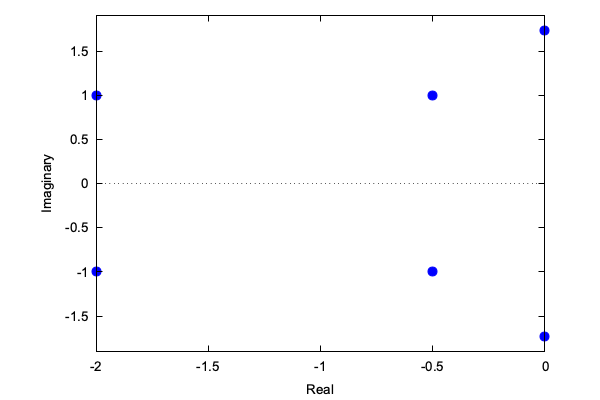
\includegraphics[width=.95\linewidth,height=.80\textheight,keepaspectratio]{question_10_b_img/question_10_b_1}\mbox{}\]

\[\tag{\% o13} 
\mbox{}
\]
%%%%%%%%%%%%%%%%
\end{document}
